\chapter{绪论}
\section{序列以及序列分类}
现实生活中会有各种各样的序列。在语音识别领域,一段语音可以被看作一段序列;在经济领域,股票的走势可以被看作是一段序列;在分子生物学领域,蛋白质、DNA也可以看成是一段序列;在网络管理中,客户端的登录活动也可以被记录成一段序列。而序列分类在现实生活中也有着广泛的应用。以语音库中的不同样本的语音为训练集,通过对需要测试的语音进行分类,可以识别出语音的来源;在医疗领域,通过对心电图序列的分类,可以得到这个疑似患者的患病信息;在信息检索的研究中,利用序列分类可将文件归类;通过蛋白质、DNA序列的分类,有助于科学家探索蛋白质、DNA的新功能\cite{Xing2010}。

一般说来,序列可以看成是事件的集合,而每一个事件可以由符号或者能比较大小的实数表示。比如一段DNA序列可以表示成$ACCCCCGT$,一段简单的时间序列可以表示成$\left\langle {0.2{\rm{,}}0.3{\rm{,}}0.5{\rm{,}}0.9{\rm{,}} \cdots } \right\rangle $,两种序列的不同之处在于实数的大小是可以度量的,而一般而言符号之间的可度量性比较差,本文主要关注的是实数序列。对于符号序列,有一类的处理方法是借鉴实数序列,比如对于蛋白质序列和DNA序列,有一种基于序列对齐的距离度量方法\cite{kajan2006application}。

对于一般的序列分类任务来说,训练集里面的序列都含有描述其类属性的标签。对于语音识别任务来说,语料库里的语音其标签是其发出者;对于文档归类任务来说,文档的标签即是其所属类别。定义$L$为标签集,$S$为待分类序列集,序列分类的任务就是通过对含有标签信息的训练集$T$的训练,得到一个可将$S$映射到$L$的分类器$C$。可以表示成$C:s \to l,s \in S,l \in L$。对于传统的分类任务来说,常用的分类器主要有$k$NN,决策树、支持向量机\cite{Wu2008}。

\section{序列分类的主要方法}
对于序列分类问题,因为其灵活性,很多的学者从不同的角度提出了大量的方法\cite{Al-Naymat2009}\cite{Keogh2000}\cite{Salvador2007}
\cite{Thrun2000}\cite{Xi2006}\cite{Ye2009}。本文主要介绍其中两种比较典型的方法,一种是基于序列距离度量的Dynamic Time Warping(DTW)方法\cite{Al-Naymat2009}\cite{Batista2011}\cite{Keogh2000}\cite{LESLIE2001}\cite{Lin2007}\cite{Salvador2007}
\cite{Xi2006},另一种是基于特征选择的shapelets方法\cite{Ye2009}。其中对DTW方法做重点介绍。
\subsection{DTW方法}
对于分类任务而言,一种广泛使用而且特别简单的方法是$k$NN方法,使用$k$NN方法时,关键的是测试数据和训练数据的亲近与否,也就是需要一种距离的度量。对于一般的实数序列,最常用的度量是欧氏距离,对于序列$s$和$s^{'}$,它们的欧式距离是:
\[dist\left( {s,{s^{'}}} \right) = \sqrt {\sum\limits_{i = 1}^L {{{\left( {s\left[ i \right] - {s^{'}}\left[ i \right]} \right)}^2}} } \]
同样地,还可以定义其他诸如街区距离,最大值距离。

但是对于序列分类而言,这些距离有很大局限性,主要体现在以下两点:
\begin{enumerate}
  \item 以上的距离度量都要求两序列长度相同,而这一点在实际问题中很难得到满足。比如在基因组分析中,很难保证基因序列的长度相同。
  \item 设想这样一种情况。在步态分析中,同一测试者的步速可能不同,或者在某时间段上存在着加速和减速。那么对于其两段步态序列,比较相似的步态之间可能会有一定的时间差,而上面的这些距离测度只会将同一时刻的步态相比较。也就是说,上面的这些距离测度不能反映出序列比较中的错位。
\end{enumerate}

而DTW方法能够很好地克服上述的两个缺点。

图\ref{fig:1}是DTW示意图,图中展现了长序列中有一定时间错位的两子序列的对齐情况\cite{Giorgino2009}。
\begin{figure}
  \centering
  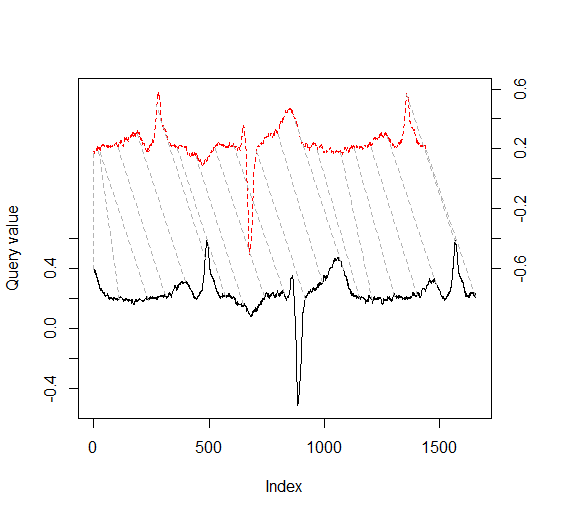
\includegraphics[width=0.6\textwidth]{./figure/two_way_plot.png}
  \caption{DTW示意图}\label{fig:1}
\end{figure}

图中的虚线表示了两序列点的对齐情况,这里对齐的两点指的是用来比较距离的两点,在传统的距离度量中,对齐的两点是索引值相同的两点。而从图中可以看出,对于DTW而言,点的对齐还参考了点邻近曲线的形态,而不仅仅局限于相同的索引,序列上的某点可以和另一个序列中的多个点对齐。因而DTW方法还能够直接处理两序列长度不同的情况。当然,对于两不同长度的时间序列,可以通过插值的方法使得序列等长,从而应用传统的距离度量方法。比如,对于两序列较短的那个,相邻点的之间可插入一定数目的点,插入点的数值可以用这两点的均值代替,以此小技巧,使得短序列扩展到与长序列长度。关于DTW的对齐规则的得到以及其他知识在后文中会详细说明。

\subsection{Shapelets方法}
Shapelets方法最早是由(Ye $et~al$ 2009)提出,作者经过大量实验,验证了该方法的优秀性\cite{Shapelets_website}。

直观来说,序列的Shapelets是该序列中最能够代表该序列的一段,如图\ref{fig:2}所示。

\begin{figure}
  \centering
  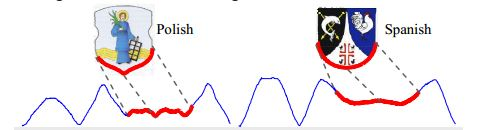
\includegraphics[width=0.6\textwidth]{./figure/shapelets.png}
  \caption{Shapelets示意图}\label{fig:2}
\end{figure}

图中的样本是两个徽章,徽章的边缘可以转换成序列。对于这两个徽章而言,徽章的下部的轮廓最能够反映该徽章的特征,因而徽章下部轮廓对应的序列是徽章序列的Shapelets。可以看出,两徽章的下部明显不同,因而可以由下部序列之间的差异,利用分类器,对徽章进行分类。在这里,一般最常用的分类器是$k$NN分类器,它简单而有效,通常取$k=1$\cite{Xi2006}

Shapelets方法有着广泛的应用,比如在植物学中,利用叶柄与叶片的角度,对植物进行分类;在考古学领域,通过对出土器件的特征部位的分类,能得到考古学发现\cite{anthropology}。
